\documentclass[10pt,a4paper]{article}
\usepackage[left=2cm,right=2cm,top=2cm,bottom=2cm]{geometry}
\usepackage[dvipsnames]{xcolor}
\usepackage[fleqn]{mathtools}
\usepackage{booktabs}
\usepackage{amsmath}
\usepackage{latexsym}
\usepackage{graphicx}
\usepackage{nccmath}
\usepackage{multicol}
\usepackage{listings}
\usepackage{tasks}
\usepackage{color}
\usepackage{float}
\usepackage{lipsum}
\usepackage{url}

\definecolor{colorIPN}{rgb}{0.5, 0.0,0.13}
\definecolor{colorESCOM}{rgb}{0.0, 0.5,1.0}
\graphicspath{ {imagenes/} }

\lstdefinestyle{macos_term}{
    backgroundcolor=\color{black},
    basicstyle=\color{white}\ttfamily\small,
    breaklines=true,
    frame=single,
    rulecolor=\color{gray}
}

\begin{document}

% --- TITLE PAGE ---
\begin{titlepage}
	\centering
	{ \huge \bfseries \color{colorIPN}{Instituto Politécnico Nacional} \par}
	{ \Large \bfseries  \color{colorESCOM}{Escuela Superior de Cómputo} \par }
	\vspace{1.5cm}
	{\huge\Large \color{colorIPN}{Web Client and Backend Development Framework}.\par}
	\vspace{2cm}
	{\huge\Large  \color{colorESCOM}{Reporte de Documentación del API con Swagger y OpenAPI}\par}
		\vspace{2.5cm}
	{\Large\itshape \color{colorIPN}{Profesor: M. en C. José Asunción Enríquez Zárate}\par} \hfill \break
	\vspace{2cm}
	{\Large\itshape \color{colorIPN}{Alumno: Luis David Martínez Martínez}\par} \hfill \break
	{\Large\itshape \color{colorIPN}{ld.martinez.117@gmail.com}\par} \hfill \break
	{\Large\itshape \color{colorIPN}{7CM3} \par}
	\vfill
	{\large \color{colorIPN}{22 de Junio, 2026}\par} 
	\vfill
\end{titlepage}

\lstset{ 
	language=Java,
	basicstyle=\small\sffamily,
	numbers=left,
	numberstyle=\tiny,
	frame=tb,
	tabsize=4,
	columns=fixed,
	showstringspaces=false,
	showtabs=false,
	keepspaces,
	commentstyle=\color{Violet},
	keywordstyle=\color{colorIPN} \bfseries,
	stringstyle=\color{colorESCOM}
}

\tableofcontents 
\pagebreak
\listoffigures
\pagebreak
\listoftables
\pagebreak
\pagenumbering{arabic}

% ################################################
\section{\color{colorIPN}{Introducción}}

La fase de integración y prueba de interfaces de programación de aplicaciones (API) REST representa una de las actividades críticas en el ciclo de vida del desarrollo de software. Tradicionalmente, la documentación de APIs se realizaba mediante documentos de texto estáticos o wikis manuales, lo que propiciaba una rápida desincronización entre la implementación real en el código fuente y las guías de consumo de los clientes web.

Para remediar esta problemática, el ecosistema de desarrollo moderno ha adoptado de forma generalizada la especificación OpenAPI (anteriormente conocida como Swagger). Swagger proporciona una suite de herramientas de código abierto basadas en una especificación común que asiste a los desarrolladores en el diseño, construcción, documentación y consumo de APIs RESTful. A través de interfaces interactivas autogeneradas, los desarrolladores de Front End pueden probar las respuestas del servidor directamente en tiempo real, agilizando el flujo operativo de los equipos de ingeniería de software.

\pagebreak

% ################################################
\section{\color{colorIPN}{Objetivo de la práctica}}

Integrar y configurar la especificación OpenAPI/Swagger en una aplicación de servicios RESTful desarrollada con el framework Spring Boot y Spring Security. Esto permitirá documentar de forma automatizada y estructurada cada uno de los endpoints de la plataforma (Habitaciones, Reservaciones, Autenticación y Archivos), detallando los tipos de datos de entrada, códigos de respuesta HTTP y políticas de seguridad, facilitando el consumo por parte del cliente Front End.

\pagebreak

% ################################################
\section{\color{colorIPN}{Conceptos}}

\subsection{\textit{\color{colorESCOM}{OpenAPI y Swagger UI}}}
OpenAPI es una especificación estandarizada para describir APIs REST sin requerir acceso al código fuente. Swagger UI, por su parte, es una herramienta que consume esta especificación para renderizar una página HTML interactiva y amigable en el navegador, permitiendo a cualquier usuario visualizar e interactuar con los recursos del API de forma inmediata.

\subsection{\textit{\color{colorESCOM}{Springdoc OpenAPI Starter}}}
Es la librería oficial recomendada para proyectos Spring Boot 3.x y superiores que automatiza la generación de la documentación. Analiza en tiempo de ejecución las anotaciones del controlador de Spring (\texttt{@RestController}, \texttt{@GetMapping}, etc.) para estructurar el archivo JSON/YAML de OpenAPI.

\subsection{\textit{\color{colorESCOM}{Anotaciones de OpenAPI}}}
\begin{itemize}
    \item \textbf{\texttt{@Tag}}: Permite agrupar operaciones por recursos lógicos (ej. Habitaciones).
    \item \textbf{\texttt{@Operation}}: Describe el propósito y comportamiento específico de un endpoint.
    \item \textbf{\texttt{@ApiResponse}}: Detalla el código de retorno HTTP (200, 201, 400, 403, 404, 500) y describe su significado en la respuesta.
\end{itemize}

\pagebreak

% ################################################
\section{\color{colorIPN}{Descripción del sistema}}

El sistema desarrollado, denominado \textbf{ReservaEasy}, consta de una arquitectura desacoplada para la administración hotelera. El módulo de backend en Spring Boot coordina la persistencia en base de datos de habitaciones y reservaciones, mientras que el módulo de seguridad garantiza que solo usuarios registrados accedan a los recursos del hotel.

\subsection{Módulos Documentados}
\begin{enumerate}
    \item \textbf{Autenticación (\texttt{/api/v1/auth}):} Permite el registro de usuarios y el inicio de sesión.
    \item \textbf{Habitaciones (\texttt{/api/v1/cuartos}):} Permite listar, crear, modificar y eliminar habitaciones.
    \item \textbf{Reservaciones (\texttt{/api/v1/reservaciones}):} Registra y cancela reservas, validando la disponibilidad de cuartos en el rango de fechas solicitado.
    \item \textbf{Archivos (\texttt{/apiArchivos/v1/archivos}):} Proporciona endpoints para subir comprobantes o imágenes a la base de datos y descargarlos.
\end{enumerate}

\pagebreak

% ################################################
\section{\color{colorIPN}{Modelo de base de datos}}

El modelo de base de datos está compuesto por las entidades principales descritas en la Tabla~\ref{tabla:BaseDatos}.

\begin{table}[htb]
    \centering
    \begin{tabular}{p{3cm}|p{6cm}|p{4cm}}\hline \hline
        Tabla     & Descripción  & Atributos Clave \\ \hline \hline
        \texttt{rooms} & Catálogo de habitaciones & \texttt{id}, \texttt{tipo}, \texttt{numero}, \texttt{precio}, \texttt{disponible} \\ \hline
        \texttt{usuarios} & Credenciales de usuarios registrados & \texttt{id}, \texttt{username}, \texttt{password}, \texttt{email} \\ \hline
        \texttt{roles} & Permisos del sistema & \texttt{id}, \texttt{nombre} (\texttt{ROLE\_ADMIN}, \texttt{ROLE\_USER}) \\ \hline
        \texttt{reservaciones} & Relación entre usuarios y habitaciones & \texttt{id}, \texttt{cuarto\_id}, \texttt{usuario\_id}, \texttt{fecha\_inicio} \\ \hline
        \texttt{archivo} & Soporte digital binario & \texttt{id\_archivo}, \texttt{nombre\_archivo}, \texttt{datos\_archivo} \\ \hline \hline
    \end{tabular}
    \caption{Esquema de entidades del sistema en base de datos}
    \label{tabla:BaseDatos}
\end{table}

\pagebreak

% ################################################
\section{\color{colorIPN}{Desarrollo}}

\subsection{\textit{\color{colorESCOM}{Configuración del Proyecto y Dependencias}}}
Para integrar la documentación se añadió la dependencia del starter oficial en el archivo \texttt{pom.xml}:
\begin{lstlisting}[language=XML]
<dependency>
    <groupId>org.springdoc</groupId>
    <artifactId>springdoc-openapi-starter-webmvc-ui</artifactId>
    <version>2.5.0</version>
</dependency>
\end{lstlisting}

\subsection{\textit{\color{colorESCOM}{Clase de Configuración ApiConfig}}}
Se creó una clase de configuración en el paquete \texttt{core/config} para personalizar los metadatos globales del API:
\begin{lstlisting}[language=Java]
@Configuration
public class ApiConfig {
    @Bean
    public OpenAPI myOpenAPI() {
        return new OpenAPI()
            .info(new Info()
                .title("API para la gestion de reservaciones")
                .version("1.0.0")
                .description("API REST para la gestion de cuartos y reservaciones")
                .contact(new Contact()
                    .name("Luis David Martinez")
                    .email("ld.martinez.117@gmail.com")));
    }
}
\end{lstlisting}

\subsection{\textit{\color{colorESCOM}{Integración en Controladores}}}
Se agregaron las anotaciones en el controlador de reservaciones:
\begin{lstlisting}[language=Java]
@RestController
@RequestMapping("/api/v1/reservaciones")
@Tag(name = "Modulo de Reservaciones", description = "Endpoints para la gestion del ciclo de vida de las reservaciones")
public class ReservationController {
    // ...
    @PostMapping
    @Operation(summary = "Crear una nueva reservacion", description = "Crea una reservacion validando disponibilidad.")
    @ApiResponses(value = {
        @ApiResponse(responseCode = "201", description = "Reservacion creada con exito"),
        @ApiResponse(responseCode = "400", description = "Fechas invalidas o conflicto de ocupacion")
    })
    public ResponseEntity<ReservationDTO> createReservation(@Valid @RequestBody CreateReservationDTO dto) {
        return ResponseEntity.status(HttpStatus.CREATED).body(reservationService.createReservation(dto));
    }
}
\end{lstlisting}

\pagebreak

% ################################################
\section{\color{colorIPN}{Resultados y Evidencias}}

Tras levantar el backend en el puerto local \texttt{8090}, accedemos al portal interactivo en la dirección:
\begin{center}
    \url{http://localhost:8090/swagger-ui/index.html}
\end{center}

\begin{figure}[H]
    \centering
    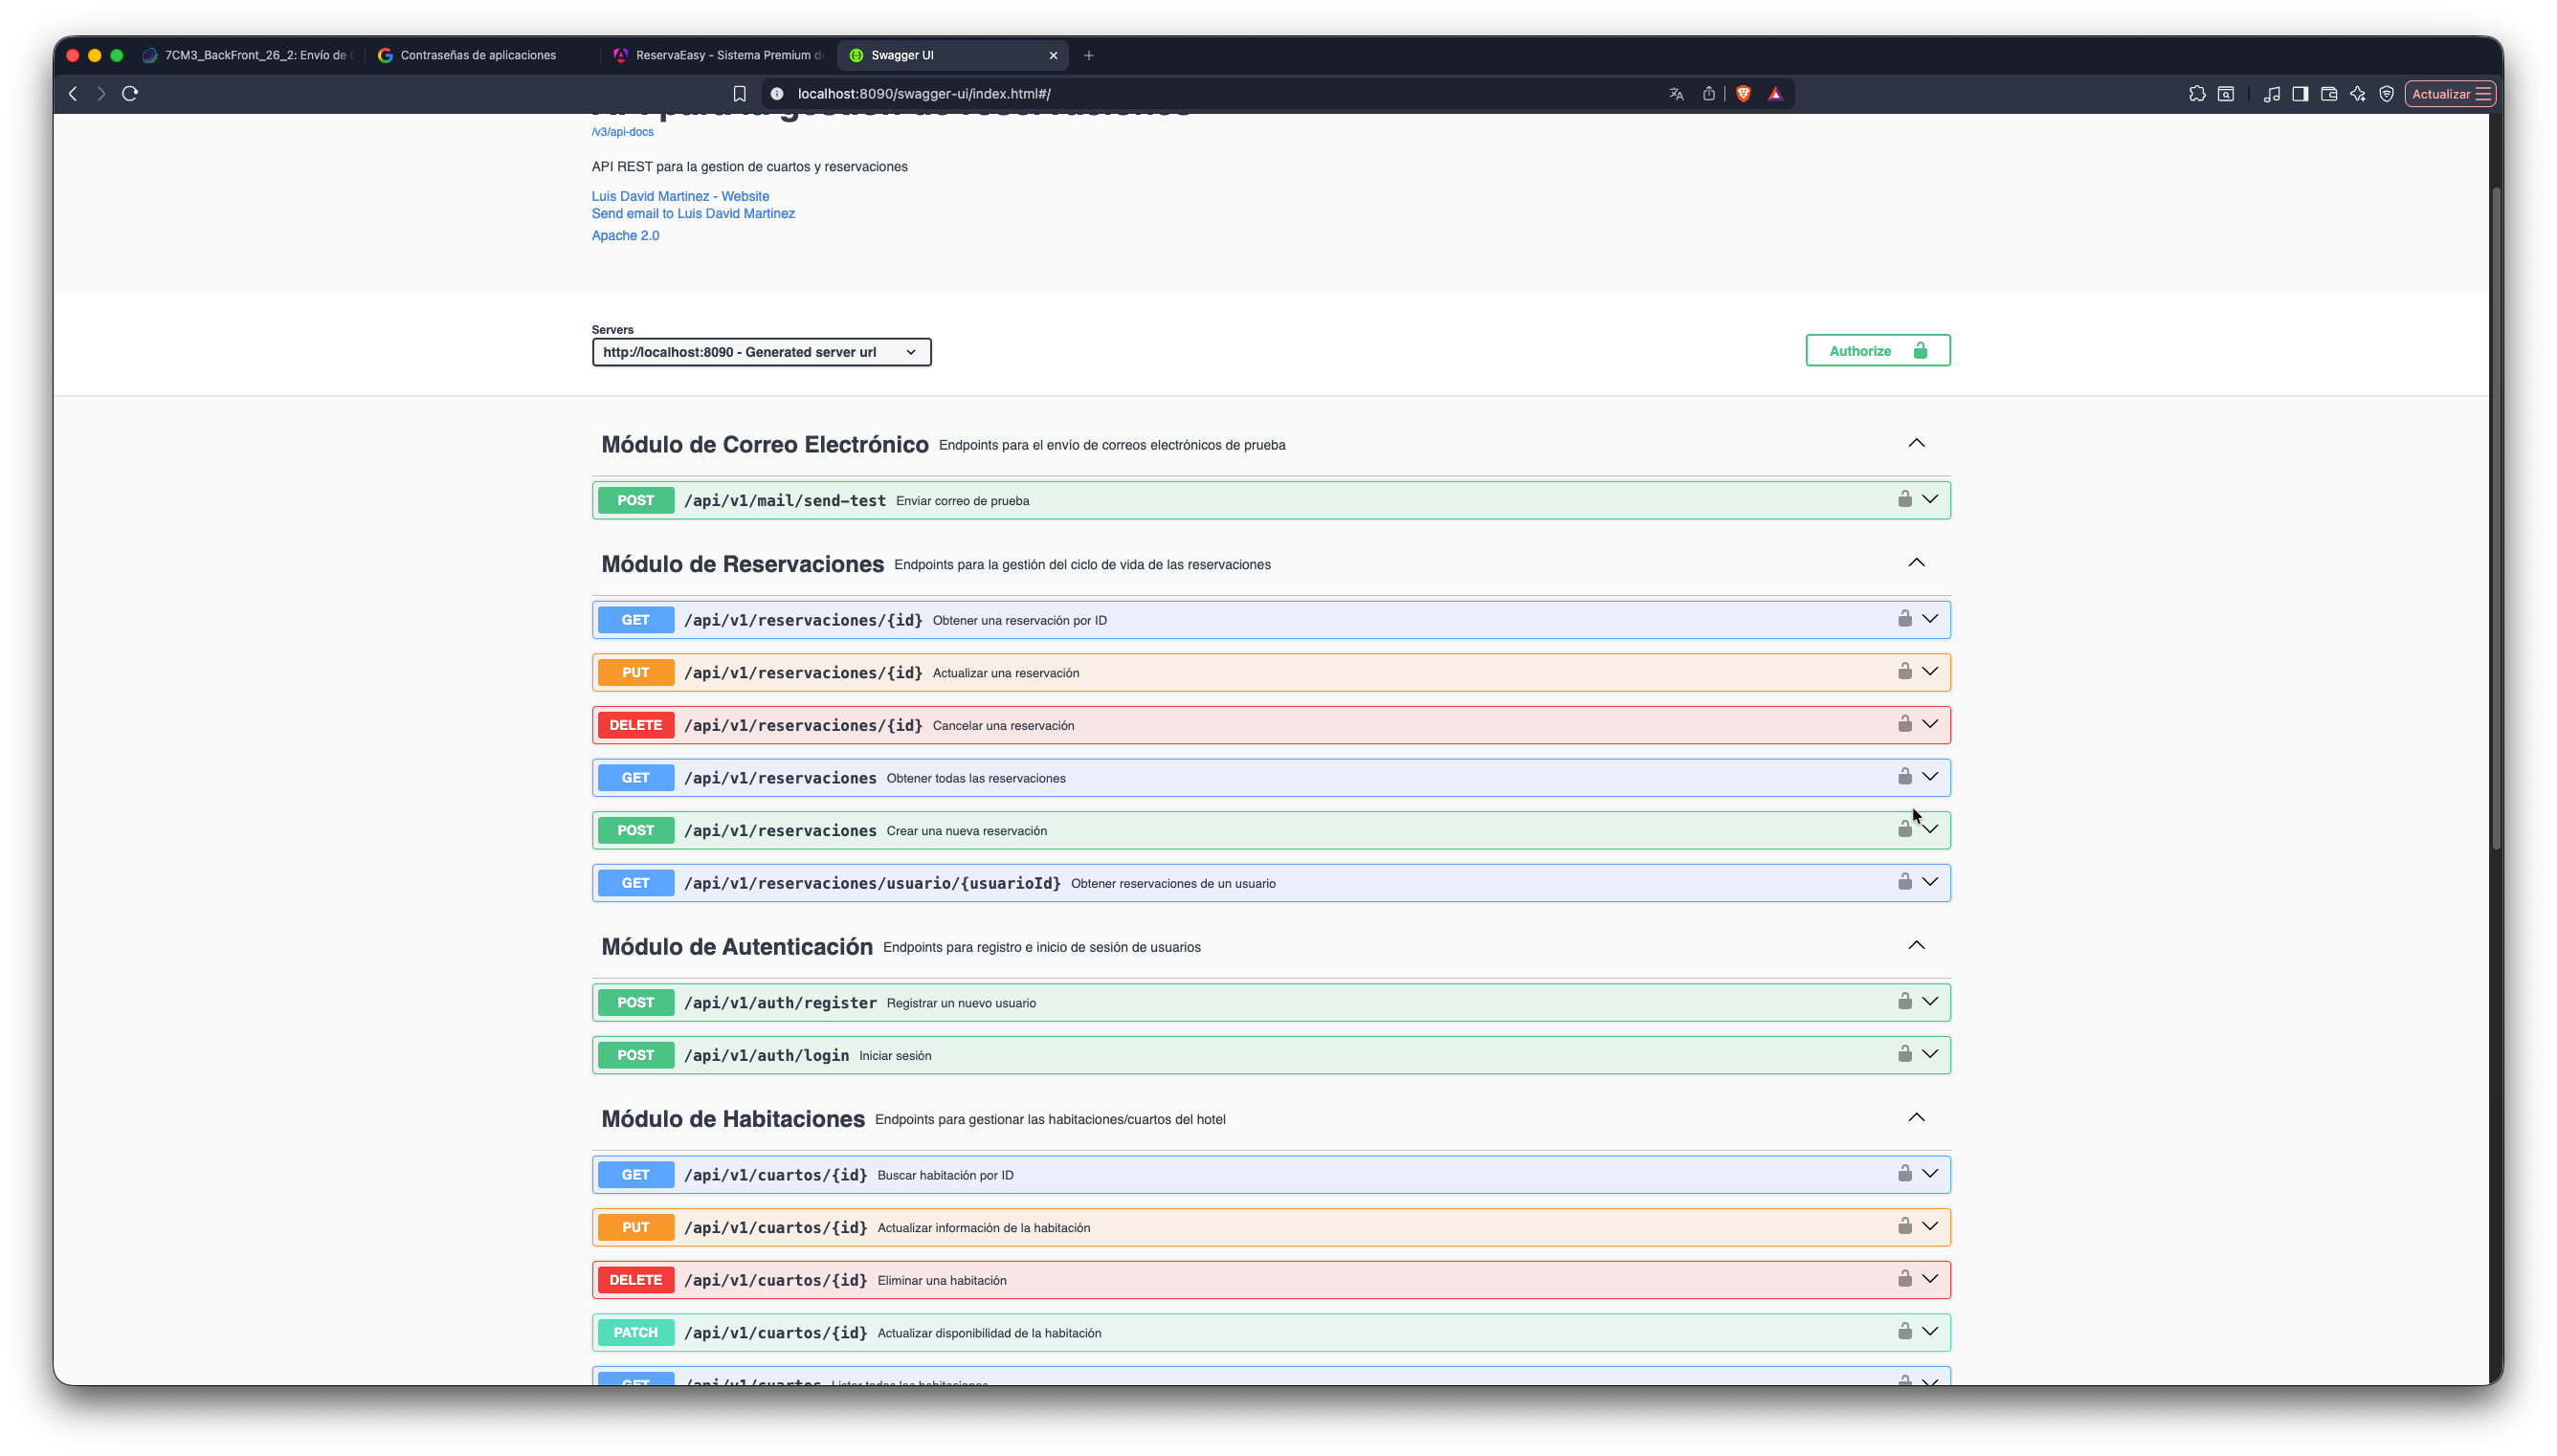
\includegraphics[width=0.75\linewidth]{imagenes/swagger_dashboard.png}
    \caption{Panel principal de Swagger UI mostrando todos los controladores documentados.}
    \label{fig:swagger_dashboard}
\end{figure}

El sistema permite ejecutar pruebas a los endpoints públicos sin credenciales, y solicita credenciales de autenticación básica HTTP para aquellos protegidos por Spring Security.
\begin{figure}[H]
    \centering
    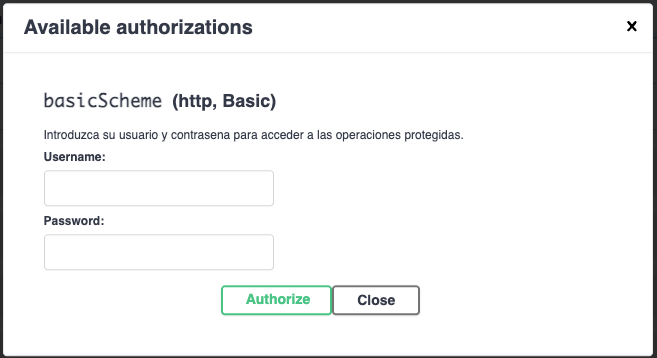
\includegraphics[width=0.75\linewidth]{swagger_auth.png}
    \caption{Modal donde se ingresan credenciales de autorización.}
    \label{fig:swagger_autorización}
\end{figure}

\begin{figure}[H]
    \centering
    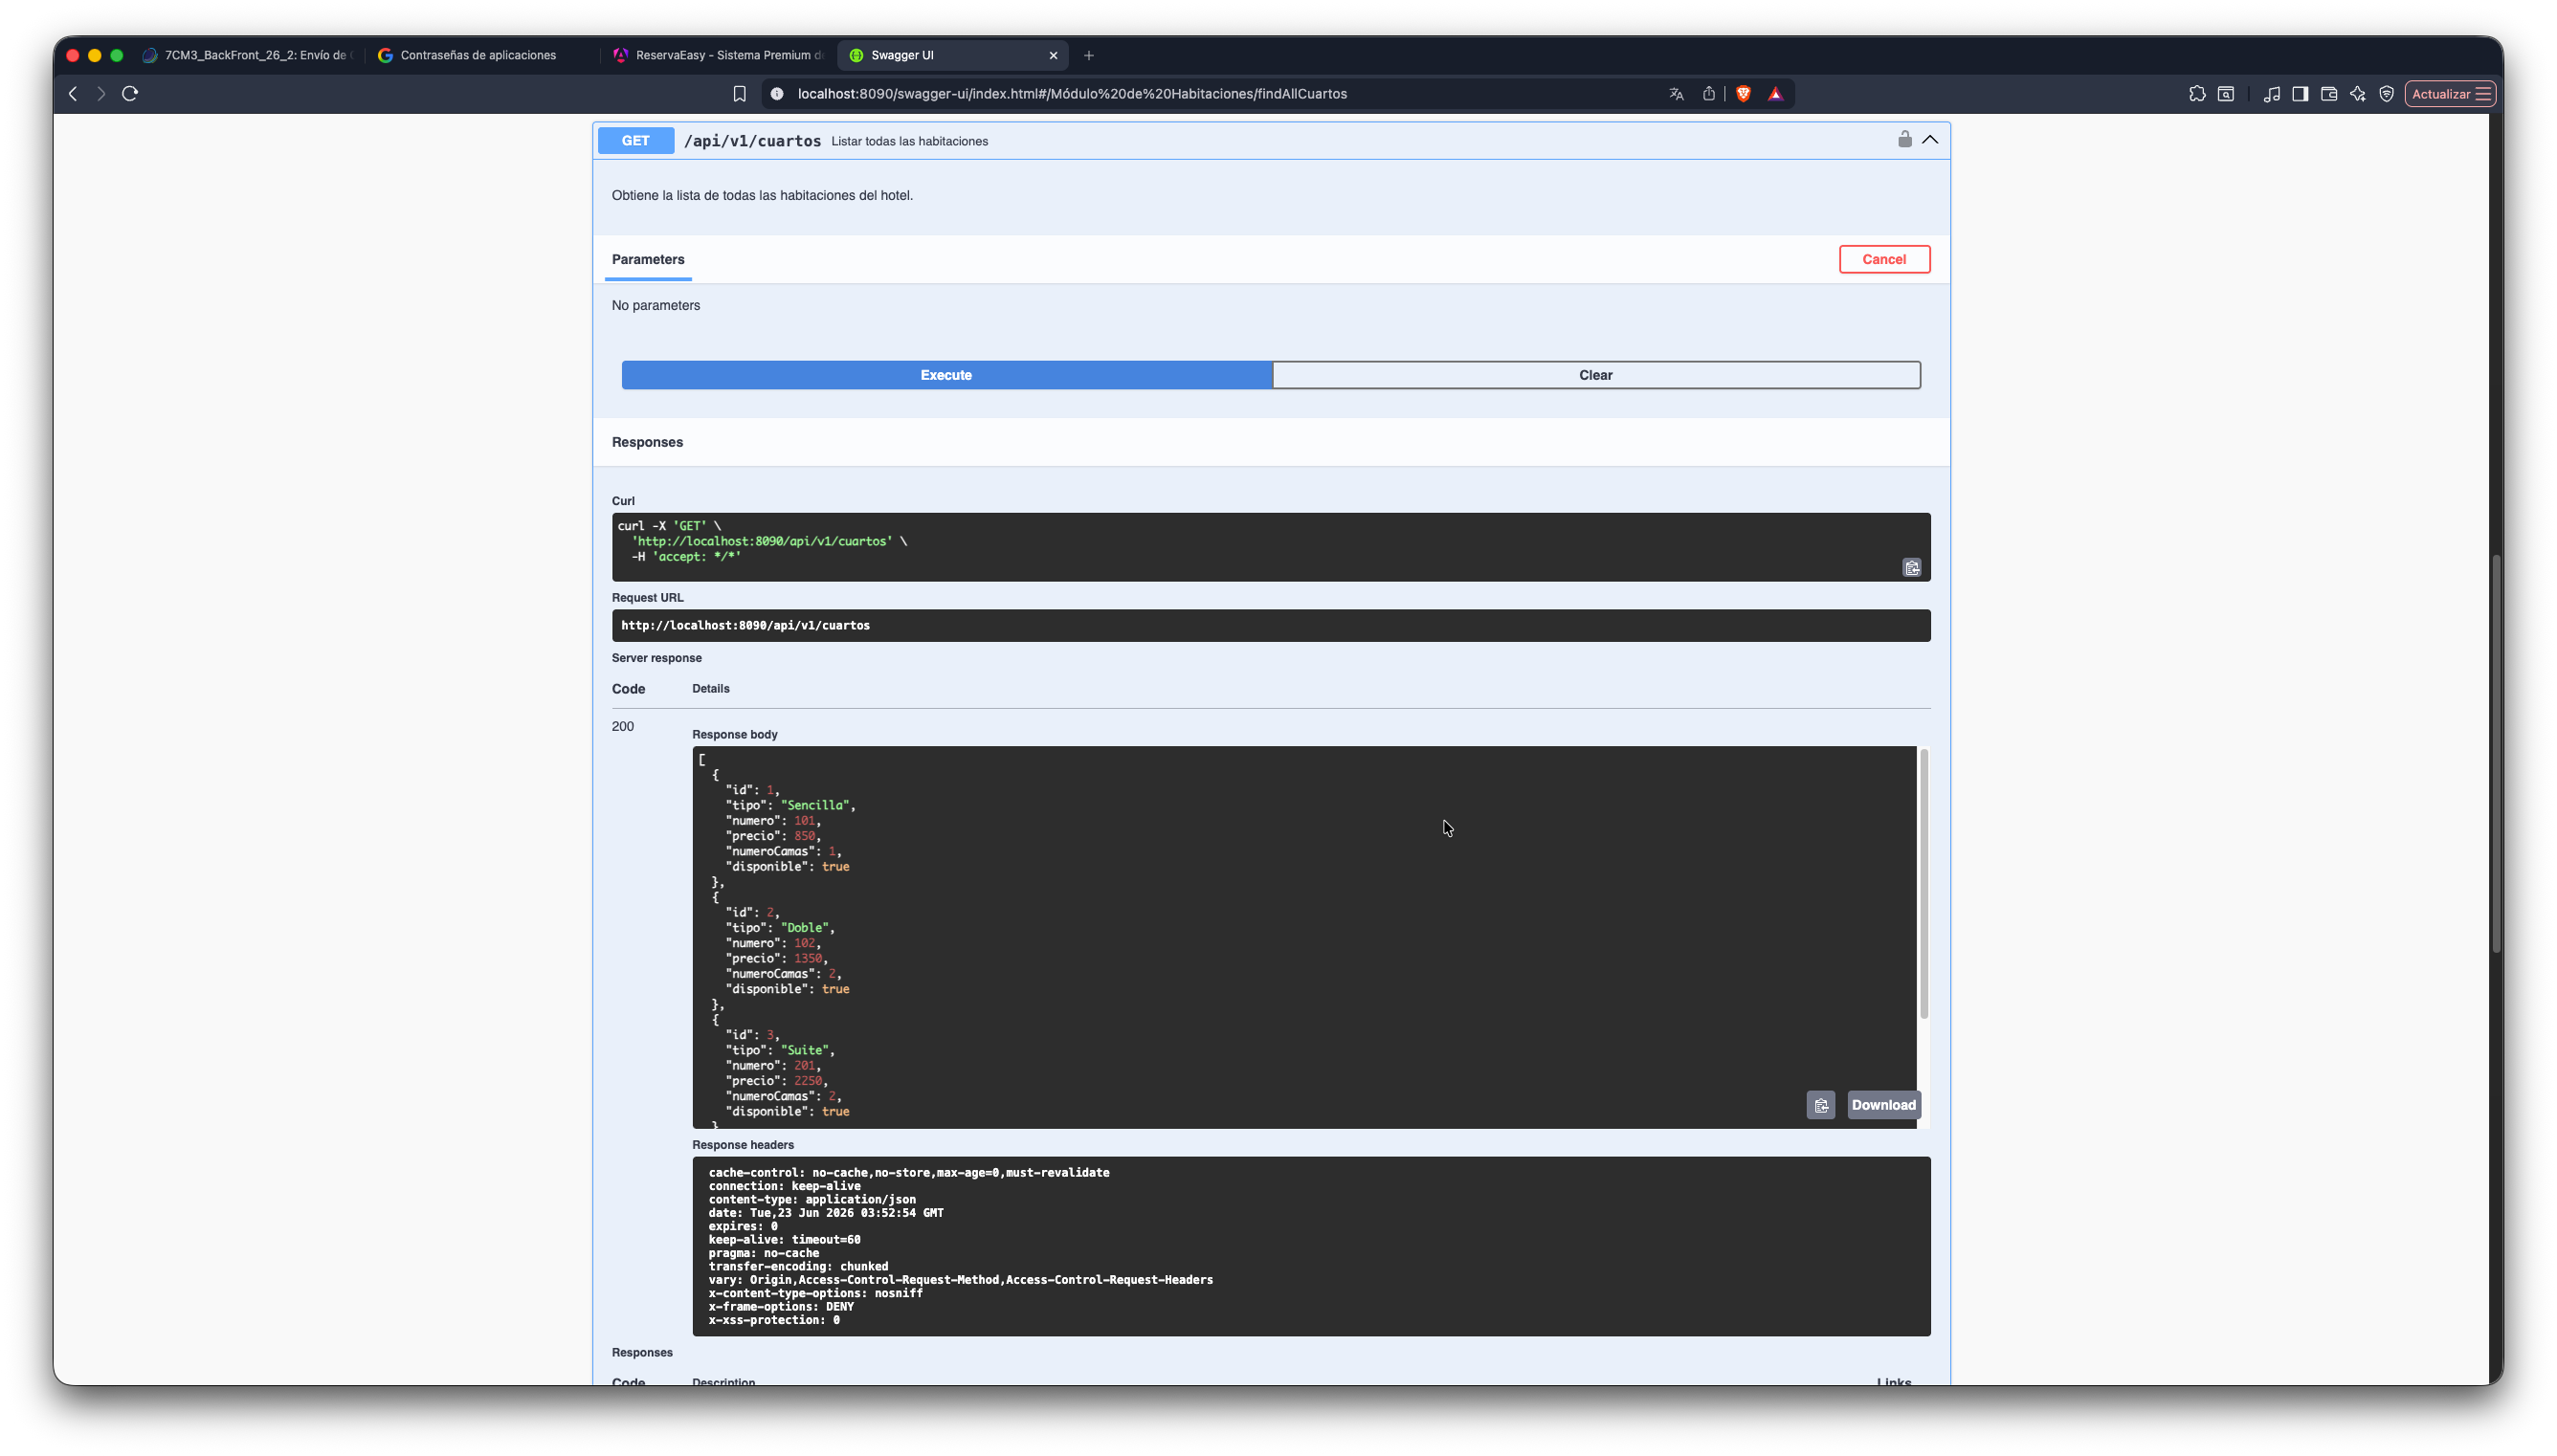
\includegraphics[width=0.75\linewidth]{swagger_pruebas.png}
    \caption{Consola de pruebas de Swagger ejecutando una consulta al catálogo de habitaciones.}
    \label{fig:swagger_pruebas}
\end{figure}

\pagebreak

% ################################################
\section{\color{colorIPN}{Conclusión}}

La documentación autogenerada con Swagger UI reduce la brecha operativa en el desarrollo full stack. Al mantener las definiciones de endpoints acopladas a las anotaciones del código Java, se garantiza que la documentación del API nunca quede obsoleta. Asimismo, proporciona un sandbox óptimo que reduce la dependencia de herramientas de desarrollo locales.

\begin{table}[htb]
    \centering
    \begin{tabular}{p{4cm}|p{2cm}|p{2cm}}\hline \hline
        Criterio     & Puntos  & Realizado \\ \hline \hline
        Portada           &  Sin  & 100\% \\ \hline 
        Objetivo          &  30\%  & 30\% \\ \hline 
        Documentación     &  40\%  & 40\% \\ \hline 
        Calidad de Descripciones & 20\%  & 20\% \\ \hline 
        Evidencias        &  10\%  & 10\% \\ \hline \hline
    \end{tabular}
    \caption{Criterios de Evaluación y Avance de la Tarea 1}
    \label{tabla:EvaluacionT1}
\end{table}

\color{colorIPN}{
	\begin{flushright}
		\textit{
			Luis David Martínez Martínez
		}
	\end{flushright} \hfill \break
}

\pagebreak

% ################################################
\section{\color{colorIPN}{Referencias Bibliográficas}}
\color{colorESCOM}{
	\begin{thebibliography}{10}
    \bibitem[Springdoc OpenAPI, 2026]{Springdoc}
    Springdoc.
    \newblock {\em Springdoc OpenAPI documentation helper.}
    \newblock Cloud Guides. Disponible en:\\ 
    \url{https://springdoc.org/}

    \bibitem[OpenAPI Initiative, 2026]{OpenAPI}
    OpenAPI.
    \newblock {\em OpenAPI Specification Standard 3.0.}
    \newblock Linux Foundation. Disponible en:\\ 
    \url{https://spec.openapis.org/oas/v3.0.3}
\end{thebibliography}
}

\end{document}
